\documentclass[letterpaper,aps,prc,superscriptaddress,nofootinbib,showpacs,floatfix]{revtex4-2}% PRC format\documentclass[12pt]
%\usepackage[super]{cite}
\usepackage{graphicx}
\usepackage{comment}
\usepackage{setspace}
\usepackage{amsmath}
\usepackage{amssymb}
%\usepackage[textwidth=16cm,textheight=22cm]{geometry}
\usepackage{color}
\usepackage{indentfirst}
\usepackage{xspace}
\usepackage{hyperref}
\usepackage{verbatim}
\usepackage{epstopdf}
\usepackage{hyperref}

%\usepackage{lineno}
%\RequirePackage{lineno}
%\setlength{\linenumbersep}{6pt}
%\linenumber\cite{weib1,weib2} 
\newcommand{\sqs}{\mbox{$\sqrt{s}$}\xspace}
\newcommand{\ee}{\mbox{$e^{+} e^{-}$}\xspace}
\newcommand{\pp}{\mbox{$pp\,(p\bar{p})$ }\xspace}
\graphicspath{ {./images/} }



\begin{document}

%\titile{
%in pp collisions at 13 TeV with Pythia 8}
\title{ Measurement of higher moments of   $\cdots$}
\author{Ankan Mukherjee} 
\email{190260008@iitb.ac.in}
\affiliation{Indian Institute of Technology Bombay, Mumbai, India}
\author{YYY}
\email{XXX@iitb.ac.in}
\affiliation{Indian Institute of Technology Bombay, Mumbai, India}
\author{ZZZ}
\email{XXX@iitb.ac.in}
\affiliation{Indian Institute of Technology Bombay, Mumbai, India}

%\email{ashutosh.kumar.pandey@cern.ch}
%\email{sadhana@phy.iitb.ac.in}


\date{\today}  



\begin{abstract}

Write a proper brief abstarct ...
\end{abstract}

\maketitle

%%%%%%%%%%%%%%%%%%%%%%%%%%%%%%%%%%%%%%%%%%%%%%%%%%%%%%%%%%%%%%%%%%%%%
\section{Introduction}
%%%%%%%%%%%%%%%%%%%%%%%%%%%%%%%%%%%%%%%%%%%%%%%%%%%%%%%%%%%%%%%%%%%%%


%The data provided is generated with Pythia 8  Monte Carlo event generator. \\
%Number of events :  2 million \\
%Collisions System :  p + p at centre of mass energy 13  TeV.\\


%Define  the variables, moments and the used formula \\

We shall be using the STAR definition. 




\section{Experimental Observations }


%1.  Distribution  of  $p_{T}$ and $<p_{T}>$ for different multiplicity classes (0-20, 20-40 etc).  \\

%All the above plots should be in logarithmic scale. \\



%2. For $|\eta < 2.5|$ (you may opt not to use any cut but mention in the text),  do the following  \\


%a.  Plot $ \sqrt{ <\Delta p_{T1} \Delta p_{T2}>} / <p_{T}> $as a function of multiplicity class. \\

%b.  Plot standardized skewness and intensive skewness as a function of multiplicity.\\

%(Use the STAR definition. Please mention if you are using any other definition.)\\

%Do not bother about errors. If possible plot the statistical errors .\\

In this section, we have plotted the histograms for the Transverse Momentum $\mathbf{pT}$ and the Mean Transverse Momentum $\mathbf{\left<pT\right>}$ of proton-proton collisions corresponding to each multiplicity class. The histogram for $\mathbf{pT}$ is then approximated using an \textbf{Exponential} fit, while that of $\mathbf{\left<pT\right>}$ has been approximated using a \textbf{Gaussian} fit. Both the quantities $\mathbf{pT}$ and $\mathbf{\left<pT\right>}$ have statistical fluctuations arising from the finite number of particles in each event. In each of the subsequent subsections corresponding to each of the 5 multiplicity classes, namely \hyperref[subsec:2040]{\textbf{pytree2040}}, \hyperref[subsec:4060]{\textbf{pytree4060}}, \hyperref[subsec:6080]{\textbf{pytree6080}}, \textbf{pytree80100} and \textbf{pytree100}, the histograms and the corresponding fits have been plotted. A logarithmic scale has been used on the \emph{y-axis} in order to emphasize the skewness of the data.

\subsection{Multiplicity Class "pytree2040"}
\label{subsec:2040}

\begin{figure}[!htb]
   \begin{minipage}{0.48\textwidth}
     \centering
     \renewcommand{\thefigure}{1a}
     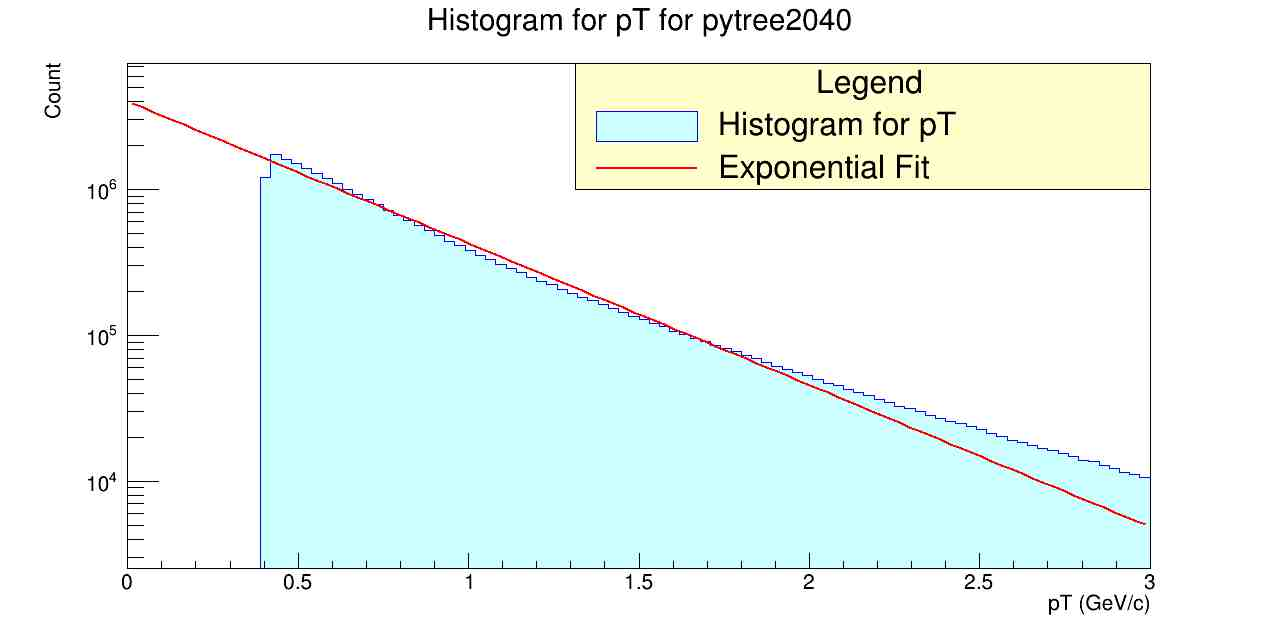
\includegraphics[width=1.1\linewidth]{pt_2040}
     \caption{Distribution of $\mathbf{pT}$ for proton-proton collision in the multiplicity class \textbf{pytree2040}. The solid line is an Exponential fit to the data.}\label{Fig:1a}
   \end{minipage}\hfill
   \begin{minipage}{0.48\textwidth}
     \centering
     \renewcommand{\thefigure}{1b}
     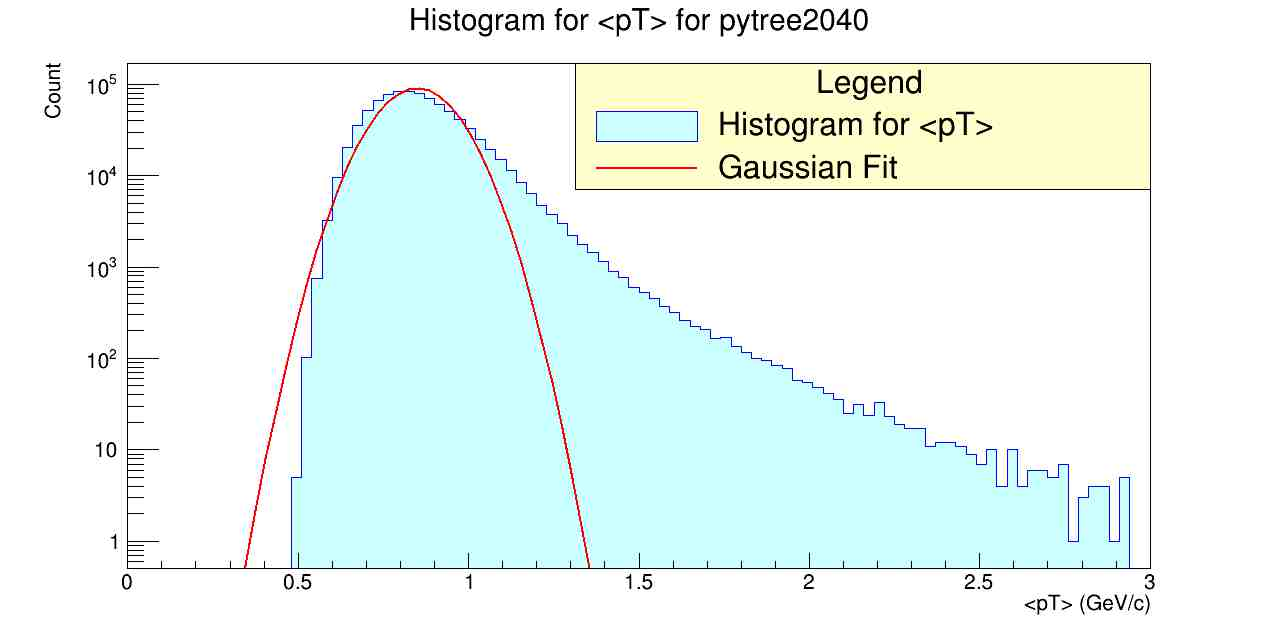
\includegraphics[width=1.1\linewidth]{/mpt_2040}
     \caption{Distribution of $\mathbf{\left<pT\right>}$ for proton-proton collision in the multiplicity class \textbf{pytree2040}. The solid line is a Gaussian fit to the data.}\label{Fig:1b}
   \end{minipage}
\end{figure}


\subsection{Multiplicity Class "pytree4060"}
\label{subsec:4060}

\subsection{Multiplicity Class "pytree6080"}
\label{subsec:6080}

\subsection{Multiplicity Class "pytree80100"}
\label{subsec:80100}

\subsection{Multiplicity Class "pytree100"}
\label{subsec:100}


\newpage
\begin{figure*}
\begin{center}
%\includegraphics[scale=0.8]{ppspectra.eps}
\caption{(Color online) Put proper captions}
\label{f1}
\end{center}
\end{figure*}



\section{Summary}

The study of  $\cdots$


\begin{thebibliography}{50}
\medskip


%\bibitem{phenixwhite} K. ~Adcox 
  %Nuclear Phys. A{\bf 757},184-283 (2005). 
  
\bibitem{alicenature} J. ~Adams {\it et al.}, (ALICE Collaboration), Nature Physics{\bf 13},535-539 (2017). 


\end{thebibliography}

\end{document}

